% You should title the file with a .tex extension (hw1.tex, for example)
\documentclass[11pt]{article}

\usepackage{hyperref}
\usepackage{amsmath}
\usepackage{mathtools}
\usepackage{amssymb}
\usepackage{wrapfig}
\usepackage{fancyhdr}
\usepackage{tikz-qtree}
\usepackage{tikz-qtree-compat}
\usepackage[normalem]{ulem}
\usepackage{tikz}
\usepackage{graphicx}
\DeclareMathOperator*{\argmin}{argmin}
\DeclareMathOperator*{\argmax}{argmax}
\setcounter{MaxMatrixCols}{20}


\oddsidemargin0cm
\topmargin-2cm     %I recommend adding these three lines to increase the 
\textwidth16.5cm   %amount of usable space on the page (and save trees)
\textheight23.5cm  

\newcommand{\question}[2] {\vspace{.25in} \hrule\vspace{0.5em}
\noindent{\bf #1: #2} \vspace{0.5em}
\hrule \vspace{.10in}}
\renewcommand{\part}[1] {\vspace{.10in} {\bf (#1)}}

\newcommand{\myname}{Sean Bittner}
\newcommand{\myandrew}{srb2201@columbia.edu}
\newcommand{\myhwnum}{12}

\setlength{\parindent}{0pt}
\setlength{\parskip}{5pt plus 1pt}
 
\DeclarePairedDelimiter\abs{\lvert}{\rvert}%
 %
\pagestyle{fancyplain}
\rhead{\fancyplain{}{\myname\\ \myandrew}}

\begin{document}

\medskip                        % Skip a "medium" amount of space
                                % (latex determines what medium is)
                                % Also try: \bigskip, \littleskip

\thispagestyle{plain}
\begin{center}                  % Center the following lines
{\Large 3.3 Discovering sufficient mechanisms of task learning} \\
Sean Bittner and John Cunningham, August 27, 2019 \\
\end{center}

\vspace{-.5cm}
\begin{wrapfigure}{b}{.58\textwidth}
  \begin{center}  
  \vspace{-.8cm}
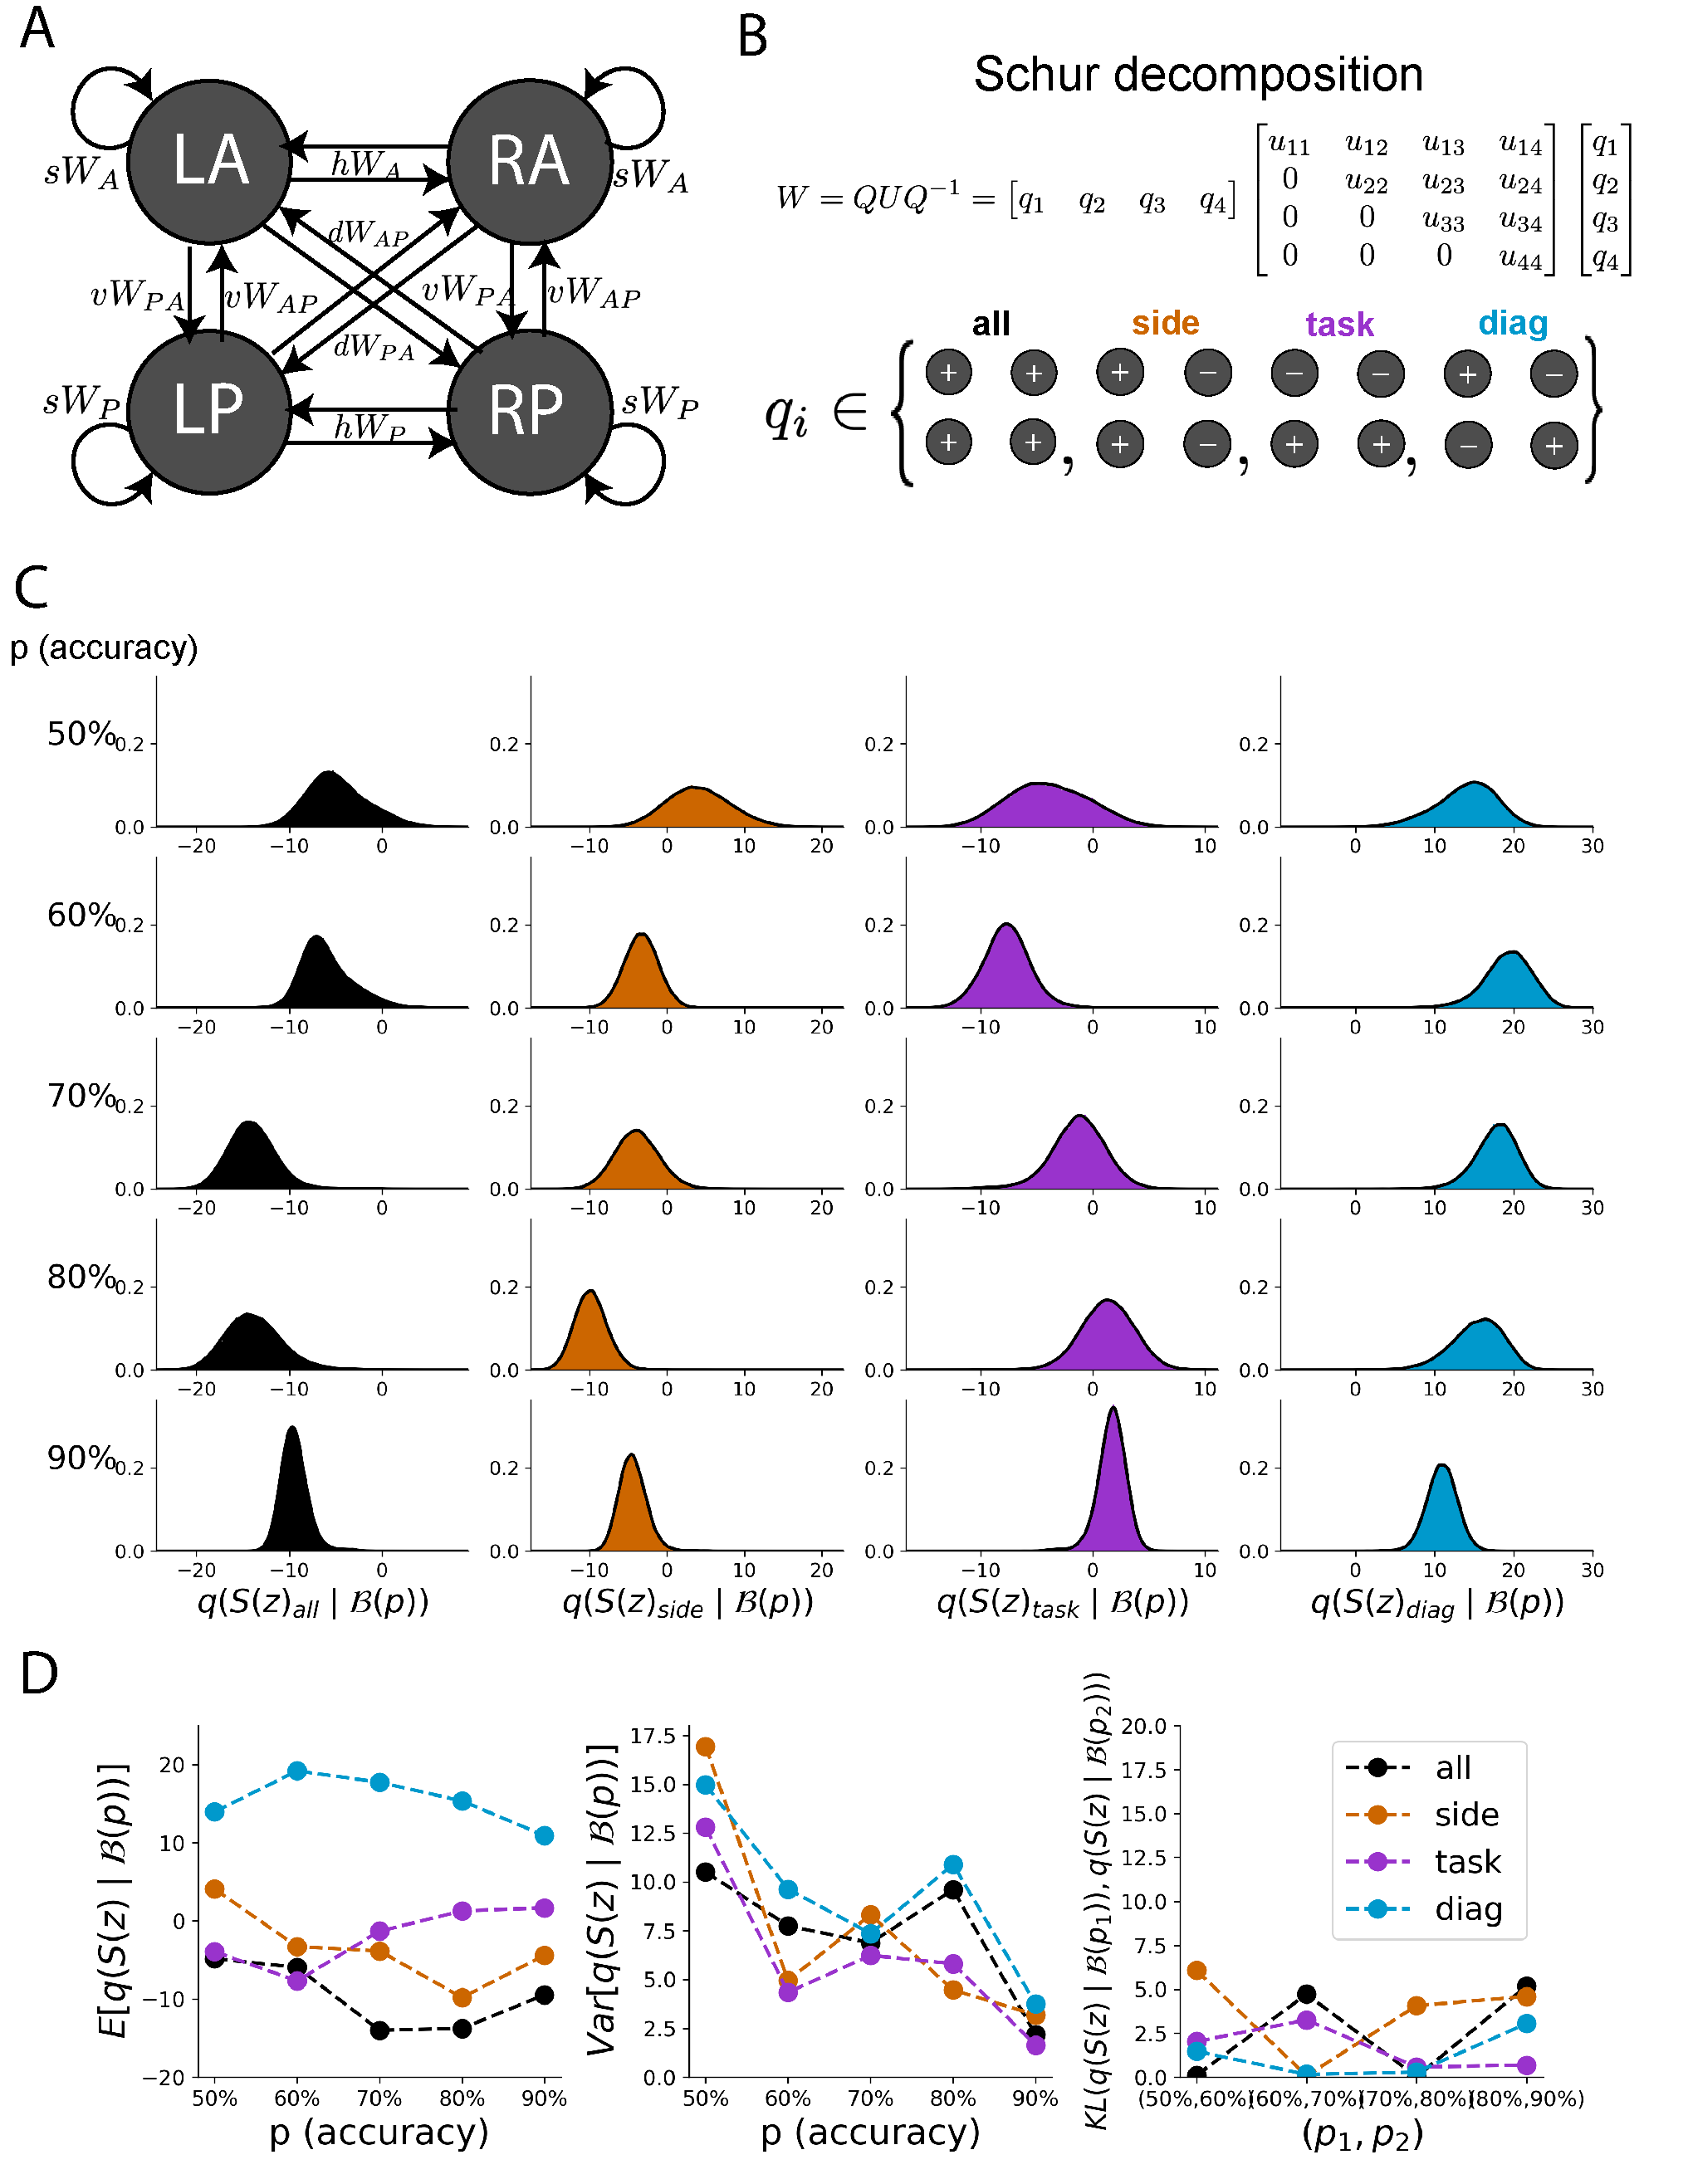
\includegraphics[scale=0.3]{SC_Fig/SC_Fig.pdf}
\vspace{-0.8cm}
\caption{\footnotesize \protectA.) Model of superior collicullus (SC). Neurons: LP - left pro, RP - right pro, LA - left anti, RA - right anti.  Parameters: sW - self, hW - horizontal, vW -vertical, dW - diagonal weights.  B.) Schur decomposition of W.  C.) DSN distribution of schur mode eigenvalues $S(z)$ with task learning.  D.) DSN means and variances (left and center, respectively) and step-wise KLs.}
\end{center}
\vspace{-1.2cm}
\end{wrapfigure}
\small

In behavioral neuroscience, model organisms are studied while performing tasks in order to investigate the underlying neural computation.  As the animal is trained, its accuracy improves via a learning process in the brain. A central challenge for theoreticians is to describe sufficient changes of model parameters that drive task performance, since such changes may indicate how the learning brain adapts.   We show that when a data-motivated, restricted dynamical model is proposed, we can use DSNs to clearly identify sufficient changes in network connectivity for task learning.

In a rapid task switching experiment, where rats are to respond right (R) or left (L) to the side of a light stimulus in the pro (P) task, and oppositely in the anti (A) task predicated by an auditory cue, neural recordings exhibited two population of neurons in each hemisphere of superior colliculus (SC) that simultaneously represented both task condition and motor response: the pro/contra and anti/ipsi neurons \cite{duan2018collicular}. We trained five DSNs on a 4-neuron model of SC proposed by Duan et al. (Fig. 1A, see Methods),  constraining the task performance in both the pro and anti tasks to an accuracy $p$ with some allowed variance fixed across chosen $p$.  We constrained the network to emit Bernoulli responses (approximately 0.0 or 1.0 on a given trial), and have winner-take-all behavior between the pro neuron populations of each hemisphere. Altogether, these DSNs, optimized to be expansive and unbiased, learned posteriors of SC model weight matrix parameters, $z = W$, conditioned on different regimes of rapid task switching performance denoted by $\mathcal{B}(p)$ (see Methods).

A convenient property of this dynamical model is that the weight matrix always has the same Schur modes (Fig. 1B), albeit variable eigenvalues for each mode.  These Schur modes have intuitive roles with respect to processing in this task, and are accordingly named the \textit{all}, \textit{side}, \textit{task}, and \textit{diag} modes.  The degree of amplification of each processing mode in a task performance regime can be examined via $q(S_\alpha(z) \mid \mathcal{B}(p))$, where $S_\alpha(z)$, $\alpha \in \{\text{all}, \text{side}, \text{task}, \text{diag} \}$, is the eigenvalue of the matching Schur mode (Fig. 1C).  

As learning progresses, the task mode is increasingly amplified, indicating the criticality of a distributed task representation at the time of stimulus presentation, (Fig. 1D, purple).  Stepping from task-naive 50\% networks to task-performing 60\% networks, there is a switch from amplified (pos. eigs.) to suppressed side mode (neg. eigs.) (Fig. 1D, orange).  Side mode suppression is also found in the regimes of greater accuracy, revealing the importance of side mode suppression in allowing a distributed task representation to exist.   Across all learning regimes, the diag mode is amplified (Fig. 1D, cyan), and the all mode is suppressed (Fig. 1D, black), which can be seen as signatures of Bernoulli winner-take-all networks.  We can conclude that side mode suppression allows rapid task switching, and that greater task-mode representation increases accuracy.


\bibliography{sc}
\bibliographystyle{unsrt}

\end{document}

